% ============================================================================
% papers/attention-selective-ner/main.tex -- DRAFT v4, 2026-09-28
% ----------------------------------------------------------------------------
% Paper 1 of 2 (author decision, 2026-09-28): ATTENTION ONLY -- everything with
% an exact null. Hidden states, output scores and probes are paper 2.
% v4: rewritten as the chain of reasoning -- each step states what we wanted to
% know, why the technique answers it, what we found, and what it left open.
% Every result is a macro from numeros.tex (numeros.py, from the tables that
% reproduzir/analise.py regenerates). Do not type a result here.
% Figures: python figuras.py.  Open decisions: \authornote{...}.
% 2026-09-28: authors and affiliations added; line numbers on for co-author review.
% ============================================================================
\documentclass[11pt,a4paper]{article}

\usepackage{iftex}
\ifXeTeX\usepackage{fontspec}\else\usepackage[utf8]{inputenc}\usepackage[T1]{fontenc}\fi
\usepackage[english]{babel}
\usepackage{amsmath,amssymb,mathtools}
\usepackage{graphicx}
\usepackage{booktabs}
\usepackage{multirow}
\usepackage{float}
\usepackage{caption}
\usepackage[dvipsnames]{xcolor}
\usepackage[round]{natbib}
\usepackage{hyperref}
\hypersetup{colorlinks=true, linkcolor=blue, citecolor=blue, urlcolor=cyan}
\usepackage[capitalise]{cleveref}
\usepackage{geometry}
\geometry{margin=2.5cm}
\usepackage{authblk}
\renewcommand\Affilfont{\small}

\newcommand{\gliner}{GLiNER}
\newcommand{\aurc}{\textsc{aurc}}
\newcommand{\authornote}[1]{\textcolor{BrickRed}{\textbf{[Open decision:} #1\textbf{]}}}
% GENERATED by numeros.py from the published tables. Do not edit.
\newcommand{\encBaseConllChance}{0.531}
\newcommand{\encBaseConllMass}{0.563}
\newcommand{\encBaseConllGeo}{0.562}
\newcommand{\encBaseConllSize}{0.494}
\newcommand{\encBaseConllSent}{0.448}
\newcommand{\encBaseConllEnr}{0.522}
\newcommand{\encBaseConllConf}{0.259}
\newcommand{\encBaseConllRsq}{0.932}
\newcommand{\encBaseConllObsExp}{0.51}
\newcommand{\encBaseGeniaChance}{0.481}
\newcommand{\encBaseGeniaMass}{0.439}
\newcommand{\encBaseGeniaGeo}{0.443}
\newcommand{\encBaseGeniaSize}{0.439}
\newcommand{\encBaseGeniaSent}{0.467}
\newcommand{\encBaseGeniaEnr}{0.514}
\newcommand{\encBaseGeniaConf}{0.316}
\newcommand{\encBaseGeniaRsq}{0.959}
\newcommand{\encBaseGeniaObsExp}{0.57}
\newcommand{\encLargeConllChance}{0.468}
\newcommand{\encLargeConllMass}{0.479}
\newcommand{\encLargeConllGeo}{0.479}
\newcommand{\encLargeConllSize}{0.422}
\newcommand{\encLargeConllSent}{0.417}
\newcommand{\encLargeConllEnr}{0.427}
\newcommand{\encLargeConllConf}{0.232}
\newcommand{\encLargeConllRsq}{0.960}
\newcommand{\encLargeConllObsExp}{0.46}
\newcommand{\encLargeGeniaChance}{0.421}
\newcommand{\encLargeGeniaMass}{0.383}
\newcommand{\encLargeGeniaGeo}{0.386}
\newcommand{\encLargeGeniaSize}{0.386}
\newcommand{\encLargeGeniaSent}{0.414}
\newcommand{\encLargeGeniaEnr}{0.457}
\newcommand{\encLargeGeniaConf}{0.278}
\newcommand{\encLargeGeniaRsq}{0.961}
\newcommand{\encLargeGeniaObsExp}{0.47}
\newcommand{\encTunedConllChance}{0.100}
\newcommand{\encTunedConllMass}{0.149}
\newcommand{\encTunedConllGeo}{0.152}
\newcommand{\encTunedConllSize}{0.119}
\newcommand{\encTunedConllSent}{0.083}
\newcommand{\encTunedConllEnr}{0.091}
\newcommand{\encTunedConllConf}{0.048}
\newcommand{\encTunedConllRsq}{0.922}
\newcommand{\encTunedConllObsExp}{0.47}
\newcommand{\encTunedGeniaChance}{0.242}
\newcommand{\encTunedGeniaMass}{0.227}
\newcommand{\encTunedGeniaGeo}{0.228}
\newcommand{\encTunedGeniaSize}{0.226}
\newcommand{\encTunedGeniaSent}{0.240}
\newcommand{\encTunedGeniaEnr}{0.245}
\newcommand{\encTunedGeniaConf}{0.110}
\newcommand{\encTunedGeniaRsq}{0.965}
\newcommand{\encTunedGeniaObsExp}{0.53}
\newcommand{\encRsqMin}{0.92}
\newcommand{\encRsqMax}{0.96}
\newcommand{\encMassGeoMaxGap}{0.004}
\newcommand{\encMassWorseThanChance}{3}
\newcommand{\encConllSentBetter}{3}
\newcommand{\encGeniaSizeBetter}{3}
\newcommand{\encObsExpMin}{0.46}
\newcommand{\encObsExpMax}{0.57}
\newcommand{\encCtwoN}{39}
\newcommand{\encCtwoFav}{9}
\newcommand{\encCtwoAdv}{6}
\newcommand{\encCtwoDeg}{0}
\newcommand{\encCtwoNul}{24}
\newcommand{\encCtwoChance}{1.0}
\newcommand{\encCthreeN}{26}
\newcommand{\encCthreeFav}{2}
\newcommand{\encCthreeAdv}{2}
\newcommand{\encCthreeDeg}{13}
\newcommand{\encCthreeNul}{22}
\newcommand{\encCthreeChance}{0.7}
\newcommand{\encCtwoBaseN}{13}
\newcommand{\encCtwoBaseFav}{4}
\newcommand{\encCtwoBaseAdv}{2}
\newcommand{\encCtwoBaseDeg}{0}
\newcommand{\encCtwoBaseNul}{7}
\newcommand{\encCtwoBaseChance}{0.3}
\newcommand{\encCthreeBaseN}{6}
\newcommand{\encCthreeBaseFav}{1}
\newcommand{\encCthreeBaseAdv}{0}
\newcommand{\encCthreeBaseDeg}{7}
\newcommand{\encCthreeBaseNul}{5}
\newcommand{\encCthreeBaseChance}{0.2}
\newcommand{\encCtwoLargeN}{13}
\newcommand{\encCtwoLargeFav}{4}
\newcommand{\encCtwoLargeAdv}{2}
\newcommand{\encCtwoLargeDeg}{0}
\newcommand{\encCtwoLargeNul}{7}
\newcommand{\encCtwoLargeChance}{0.3}
\newcommand{\encCthreeLargeN}{13}
\newcommand{\encCthreeLargeFav}{1}
\newcommand{\encCthreeLargeAdv}{2}
\newcommand{\encCthreeLargeDeg}{0}
\newcommand{\encCthreeLargeNul}{10}
\newcommand{\encCthreeLargeChance}{0.3}
\newcommand{\encCtwoTunedN}{13}
\newcommand{\encCtwoTunedFav}{1}
\newcommand{\encCtwoTunedAdv}{2}
\newcommand{\encCtwoTunedDeg}{0}
\newcommand{\encCtwoTunedNul}{10}
\newcommand{\encCtwoTunedChance}{0.3}
\newcommand{\encCthreeTunedN}{7}
\newcommand{\encCthreeTunedFav}{0}
\newcommand{\encCthreeTunedAdv}{0}
\newcommand{\encCthreeTunedDeg}{6}
\newcommand{\encCthreeTunedNul}{7}
\newcommand{\encCthreeTunedChance}{0.2}
\newcommand{\ctwoGeniaBaseD}{-0.0039}
\newcommand{\ctwoGeniaBaseLo}{-0.0071}
\newcommand{\ctwoGeniaBaseHi}{-0.0009}
\newcommand{\ctwoGeniaLargeD}{-0.0036}
\newcommand{\ctwoGeniaLargeLo}{-0.0067}
\newcommand{\ctwoGeniaLargeHi}{-0.0006}
\newcommand{\ctwoGeniaTunedD}{-0.0014}
\newcommand{\ctwoGeniaTunedLo}{-0.0042}
\newcommand{\ctwoGeniaTunedHi}{+0.0014}
\newcommand{\encTtwoN}{9}
\newcommand{\encTtwoFav}{0}
\newcommand{\encTtwoAdv}{8}
\newcommand{\encTtwoDeg}{3}
\newcommand{\encTtwoNul}{1}
\newcommand{\encTtwoChance}{0.2}
\newcommand{\encTthreeN}{17}
\newcommand{\encTthreeFav}{0}
\newcommand{\encTthreeAdv}{15}
\newcommand{\encTthreeDeg}{3}
\newcommand{\encTthreeNul}{2}
\newcommand{\encTthreeChance}{0.4}
\newcommand{\encTfourN}{15}
\newcommand{\encTfourFav}{0}
\newcommand{\encTfourAdv}{0}
\newcommand{\encTfourDeg}{8}
\newcommand{\encTfourNul}{15}
\newcommand{\encTfourChance}{0.4}
\newcommand{\famLargeAttN}{40}
\newcommand{\famLargeAttFav}{0}
\newcommand{\famLargeAttAdv}{38}
\newcommand{\famLargeAttDeg}{0}
\newcommand{\famLargeAttNul}{2}
\newcommand{\famLargeAttChance}{1.0}
\newcommand{\famLargeHidN}{22}
\newcommand{\famLargeHidFav}{0}
\newcommand{\famLargeHidAdv}{18}
\newcommand{\famLargeHidDeg}{0}
\newcommand{\famLargeHidNul}{4}
\newcommand{\famLargeHidChance}{0.6}
\newcommand{\famLargeLogitN}{28}
\newcommand{\famLargeLogitFav}{3}
\newcommand{\famLargeLogitAdv}{10}
\newcommand{\famLargeLogitDeg}{16}
\newcommand{\famLargeLogitNul}{15}
\newcommand{\famLargeLogitChance}{0.7}
\newcommand{\famLargeGeoN}{24}
\newcommand{\famLargeGeoFav}{0}
\newcommand{\famLargeGeoAdv}{6}
\newcommand{\famLargeGeoDeg}{0}
\newcommand{\famLargeGeoNul}{18}
\newcommand{\famLargeGeoChance}{0.6}
\newcommand{\famLargeAllN}{114}
\newcommand{\famLargeAllFav}{3}
\newcommand{\famLargeAllAdv}{72}
\newcommand{\famLargeAllDeg}{16}
\newcommand{\famLargeAllNul}{39}
\newcommand{\famLargeAllChance}{2.9}
\newcommand{\famLargeFavSignals}{logit\_margin}
\newcommand{\famTunedAttN}{31}
\newcommand{\famTunedAttFav}{0}
\newcommand{\famTunedAttAdv}{27}
\newcommand{\famTunedAttDeg}{12}
\newcommand{\famTunedAttNul}{4}
\newcommand{\famTunedAttChance}{0.8}
\newcommand{\famTunedHidN}{24}
\newcommand{\famTunedHidFav}{0}
\newcommand{\famTunedHidAdv}{21}
\newcommand{\famTunedHidDeg}{9}
\newcommand{\famTunedHidNul}{3}
\newcommand{\famTunedHidChance}{0.6}
\newcommand{\famTunedLogitN}{17}
\newcommand{\famTunedLogitFav}{2}
\newcommand{\famTunedLogitAdv}{2}
\newcommand{\famTunedLogitDeg}{20}
\newcommand{\famTunedLogitNul}{13}
\newcommand{\famTunedLogitChance}{0.4}
\newcommand{\famTunedGeoN}{18}
\newcommand{\famTunedGeoFav}{0}
\newcommand{\famTunedGeoAdv}{10}
\newcommand{\famTunedGeoDeg}{10}
\newcommand{\famTunedGeoNul}{8}
\newcommand{\famTunedGeoChance}{0.5}
\newcommand{\famTunedAllN}{90}
\newcommand{\famTunedAllFav}{2}
\newcommand{\famTunedAllAdv}{60}
\newcommand{\famTunedAllDeg}{51}
\newcommand{\famTunedAllNul}{28}
\newcommand{\famTunedAllChance}{2.2}
\newcommand{\famTunedFavSignals}{logit\_margin}
\newcommand{\ftFoneGeniaBefore}{0.560}
\newcommand{\ftFoneGeniaAfter}{0.768}
\newcommand{\ftFoneConllBefore}{0.673}
\newcommand{\ftFoneConllAfter}{0.970}
\newcommand{\pilotFloorGeniaD}{-0.0419}
\newcommand{\pilotFloorGeniaLo}{-0.0575}
\newcommand{\pilotFloorGeniaHi}{-0.0267}
\newcommand{\pilotFloorConllD}{+0.0319}
\newcommand{\pilotFloorConllLo}{+0.0186}
\newcommand{\pilotFloorConllHi}{+0.0442}
\newcommand{\periReadings}{2496}
\newcommand{\periGeniaZeroWeight}{24}
\newcommand{\periGeniaMaxWeight}{0.37}
\newcommand{\periGeniaBestDelta}{-0.0178}
\newcommand{\periGeniaSizeCorr}{0.64}
\newcommand{\periConllZeroWeight}{79}
\newcommand{\periConllMaxWeight}{0.06}
\newcommand{\periConllBestDelta}{-0.0081}
\newcommand{\periConllSizeCorr}{0.55}
\newcommand{\decRsqMin}{0.83}
\newcommand{\decRsqMax}{0.88}
\newcommand{\decSmallConllChance}{0.188}
\newcommand{\decSmallConllMass}{0.217}
\newcommand{\decSmallConllGeo}{0.232}
\newcommand{\decSmallConllConf}{0.068}
\newcommand{\decSmallConllProbe}{0.052}
\newcommand{\decSmallConllSize}{0.193}
\newcommand{\decSmallGeniaChance}{0.243}
\newcommand{\decSmallGeniaMass}{0.252}
\newcommand{\decSmallGeniaGeo}{0.255}
\newcommand{\decSmallGeniaConf}{0.153}
\newcommand{\decSmallGeniaProbe}{0.143}
\newcommand{\decSmallGeniaSize}{0.248}
\newcommand{\decLargeConllChance}{0.181}
\newcommand{\decLargeConllMass}{0.241}
\newcommand{\decLargeConllGeo}{0.247}
\newcommand{\decLargeConllConf}{0.058}
\newcommand{\decLargeConllProbe}{0.049}
\newcommand{\decLargeConllSize}{0.190}
\newcommand{\decLargeGeniaChance}{0.250}
\newcommand{\decLargeGeniaMass}{0.263}
\newcommand{\decLargeGeniaGeo}{0.265}
\newcommand{\decLargeGeniaConf}{0.166}
\newcommand{\decLargeGeniaProbe}{0.150}
\newcommand{\decLargeGeniaSize}{0.257}
\newcommand{\decMassWorseThanChance}{4}
\newcommand{\decSmallConllMassCal}{0.165}
\newcommand{\decSmallConllGeoCal}{0.140}
\newcommand{\decSmallGeniaMassCal}{0.240}
\newcommand{\decSmallGeniaGeoCal}{0.231}
\newcommand{\decLargeConllMassCal}{0.149}
\newcommand{\decLargeConllGeoCal}{0.131}
\newcommand{\decLargeGeniaMassCal}{0.244}
\newcommand{\decLargeGeniaGeoCal}{0.233}
\newcommand{\decCalGapMin}{0.009}
\newcommand{\decCalGapMax}{0.025}
\newcommand{\decCalGapAdv}{4}
\newcommand{\decRawGapMin}{-0.014}
\newcommand{\decRawGapMax}{-0.002}
\newcommand{\rrDecMassCalMin}{1}
\newcommand{\rrDecMassCalMax}{17}
\newcommand{\rrDecGeoCalMin}{5}
\newcommand{\rrDecGeoCalMax}{28}
\newcommand{\decCalBothBeatChance}{4}
\newcommand{\decUnsupPooledN}{48}
\newcommand{\decUnsupPooledFav}{0}
\newcommand{\decUnsupPooledAdv}{48}
\newcommand{\decUnsupPooledDeg}{0}
\newcommand{\decUnsupPooledNul}{0}
\newcommand{\decUnsupPooledChance}{1.2}
\newcommand{\decUnsupAllN}{312}
\newcommand{\decUnsupAllFav}{1}
\newcommand{\decUnsupAllAdv}{265}
\newcommand{\decUnsupAllDeg}{0}
\newcommand{\decUnsupAllNul}{46}
\newcommand{\decUnsupAllChance}{7.8}
\newcommand{\decCtwoN}{4}
\newcommand{\decCtwoFav}{0}
\newcommand{\decCtwoAdv}{4}
\newcommand{\decCtwoDeg}{0}
\newcommand{\decCtwoNul}{0}
\newcommand{\decCtwoChance}{0.1}
\newcommand{\decCthreeN}{1}
\newcommand{\decCthreeFav}{0}
\newcommand{\decCthreeAdv}{0}
\newcommand{\decCthreeDeg}{3}
\newcommand{\decCthreeNul}{1}
\newcommand{\decCthreeChance}{0.0}
\newcommand{\decUnsupLoadN}{213}
\newcommand{\decUnsupLoadFav}{0}
\newcommand{\decUnsupLoadAdv}{167}
\newcommand{\decUnsupLoadDeg}{64}
\newcommand{\decUnsupLoadNul}{46}
\newcommand{\decUnsupLoadChance}{5.3}
\newcommand{\decProbeHidConfN}{4}
\newcommand{\decProbeHidConfFav}{3}
\newcommand{\decProbeHidConfAdv}{0}
\newcommand{\decProbeHidConfDeg}{0}
\newcommand{\decProbeHidConfNul}{1}
\newcommand{\decProbeHidConfChance}{0.1}
\newcommand{\decProbeHidAggN}{4}
\newcommand{\decProbeHidAggFav}{1}
\newcommand{\decProbeHidAggAdv}{0}
\newcommand{\decProbeHidAggDeg}{0}
\newcommand{\decProbeHidAggNul}{3}
\newcommand{\decProbeHidAggChance}{0.1}
\newcommand{\decProbeAttConfN}{4}
\newcommand{\decProbeAttConfFav}{1}
\newcommand{\decProbeAttConfAdv}{0}
\newcommand{\decProbeAttConfDeg}{0}
\newcommand{\decProbeAttConfNul}{3}
\newcommand{\decProbeAttConfChance}{0.1}
\newcommand{\decProbeAttAggN}{4}
\newcommand{\decProbeAttAggFav}{0}
\newcommand{\decProbeAttAggAdv}{1}
\newcommand{\decProbeAttAggDeg}{0}
\newcommand{\decProbeAttAggNul}{3}
\newcommand{\decProbeAttAggChance}{0.1}
\newcommand{\decAdOneN}{104}
\newcommand{\decAdOneFav}{87}
\newcommand{\decAdOneAdv}{0}
\newcommand{\decAdOneDeg}{0}
\newcommand{\decAdOneNul}{17}
\newcommand{\decAdOneChance}{2.6}
\newcommand{\decHallucMin}{22}
\newcommand{\decHallucMax}{80}
\newcommand{\nSentGenia}{1,854}
\newcommand{\nSentConll}{3,453}
\newcommand{\declCalFrac}{30}
\newcommand{\declResamples}{2,000}
\newcommand{\declSeed}{42}
\newcommand{\declQualityGrid}{0.70, 0.80, 0.90, 0.95}
\newcommand{\nDeclarations}{26}
\newcommand{\rrEncConfMin}{34}
\newcommand{\rrEncConfMax}{54}
\newcommand{\rrDecConfMin}{33}
\newcommand{\rrDecConfMax}{68}
\newcommand{\rrEncMassMin}{-49}
\newcommand{\rrEncMassMax}{9}
\newcommand{\rrDecMassMin}{-33}
\newcommand{\rrDecMassMax}{-3}
\newcommand{\rrDecProbeMin}{40}
\newcommand{\rrDecProbeMax}{73}
\newcommand{\rrSizeGeniaMin}{6}
\newcommand{\rrSizeGeniaMax}{9}
\newcommand{\rrSentGeniaMin}{1}
\newcommand{\rrSentGeniaMax}{3}
\newcommand{\rrGeoGeniaMin}{6}
\newcommand{\rrGeoGeniaMax}{8}
\newcommand{\rrSizeConllMin}{-19}
\newcommand{\rrSizeConllMax}{10}
\newcommand{\rrSentConllMin}{11}
\newcommand{\rrSentConllMax}{17}
\newcommand{\rrGeoConllMin}{-51}
\newcommand{\rrGeoConllMax}{-2}
\newcommand{\rrDecEntConllMin}{27}
\newcommand{\rrDecEntConllMax}{30}
\newcommand{\rrDecConfConllMin}{64}
\newcommand{\rrDecConfConllMax}{68}
\newcommand{\rrBestAttentionMax}{30}
\newcommand{\rrBestAttentionMin}{-6}
\newcommand{\rrEncBestAttentionMax}{12}
\newcommand{\rrBestHiddenMax}{9}
\newcommand{\rrBestHiddenMin}{-16}
\newcommand{\rrEncBestHiddenMax}{9}
\newcommand{\rrBestOutputMax}{61}
\newcommand{\rrBestOutputMin}{34}
\newcommand{\rrEncBestOutputMax}{61}
\newcommand{\rrHiddenBelowChance}{6}
\newcommand{\rrHiddenCells}{8}
\newcommand{\rrGeniaMassBase}{9}
\newcommand{\rrGeniaConfBase}{34}
\newcommand{\rrLogitConllMin}{52}
\newcommand{\rrLogitConllMax}{61}
\newcommand{\rrConfConllMin}{50}
\newcommand{\rrConfConllMax}{52}
\newcommand{\cthreeMaxAbs}{0.007}
\newcommand{\cthreeZeroPairs}{2}
\newcommand{\cthreePairs}{6}
\newcommand{\cthreeMaxRel}{3}
\newcommand{\loadTunedGeniaConf}{46}
\newcommand{\loadTunedGeniaMass}{100}
\newcommand{\decAttPooledN}{24}
\newcommand{\decAttPooledFav}{0}
\newcommand{\decAttPooledAdv}{24}
\newcommand{\decAttPooledDeg}{0}
\newcommand{\decAttPooledNul}{0}
\newcommand{\decAttPooledChance}{0.6}
\newcommand{\decAttPooledConfN}{12}
\newcommand{\decAttPooledConfFav}{0}
\newcommand{\decAttPooledConfAdv}{12}
\newcommand{\decAttPooledConfDeg}{0}
\newcommand{\decAttPooledConfNul}{0}
\newcommand{\decAttPooledConfChance}{0.3}
\newcommand{\decAttPooledAggN}{12}
\newcommand{\decAttPooledAggFav}{0}
\newcommand{\decAttPooledAggAdv}{12}
\newcommand{\decAttPooledAggDeg}{0}
\newcommand{\decAttPooledAggNul}{0}
\newcommand{\decAttPooledAggChance}{0.3}
\newcommand{\decAttLoadN}{122}
\newcommand{\decAttLoadFav}{0}
\newcommand{\decAttLoadAdv}{94}
\newcommand{\decAttLoadDeg}{30}
\newcommand{\decAttLoadNul}{28}
\newcommand{\decAttLoadChance}{3.1}
\newcommand{\rrEncEntMin}{-1}
\newcommand{\rrEncEntMax}{12}
\newcommand{\rrEncMaxMin}{-8}
\newcommand{\rrEncMaxMax}{-5}
\newcommand{\rrEncEmitMin}{-23}
\newcommand{\rrEncEmitMax}{2}
\newcommand{\rrDecEntMin}{4}
\newcommand{\rrDecEntMax}{30}
\newcommand{\rrDecMaxMin}{-47}
\newcommand{\rrDecMaxMax}{-8}
\newcommand{\rrAttBelowConfMin}{25}
\newcommand{\nAttCells}{10}
\newcommand{\strataCtwoN}{33}
\newcommand{\strataCtwoFav}{7}
\newcommand{\strataCtwoAdv}{6}
\newcommand{\strataCtwoMaxAbs}{0.049}
\newcommand{\strataCtwoNonDeg}{33}
\newcommand{\strataCtwoChance}{0.83}
\newcommand{\strataCtwoNAll}{39}
\newcommand{\strataCthreeN}{33}
\newcommand{\strataCthreeFav}{2}
\newcommand{\strataCthreeAdv}{1}
\newcommand{\strataCthreeMaxAbs}{0.014}
\newcommand{\strataCthreeNonDeg}{22}
\newcommand{\strataCthreeChance}{0.55}
\newcommand{\strataCthreeNAll}{39}
\newcommand{\cthreeKoneConllBaseD}{-0.0029}
\newcommand{\cthreeKoneConllLargeD}{-0.0141}
\newcommand{\cthreeKoneConllTunedD}{0.0000}
\newcommand{\periGeniaMedDelta}{-0.0016}
\newcommand{\periGeniaQuartDelta}{-0.0053}
\newcommand{\periGeniaQuartDeltaAbs}{0.0053}
\newcommand{\periGeniaMedWeight}{0.02}
\newcommand{\periConllMedDelta}{0.0000}
\newcommand{\periConllQuartDelta}{0.0000}
\newcommand{\periConllQuartDeltaAbs}{0.0000}
\newcommand{\periConllMedWeight}{0.00}
\newcommand{\decStrataCtwoN}{22}
\newcommand{\decStrataCtwoFav}{1}
\newcommand{\decStrataCtwoAdv}{7}
\newcommand{\decStrataCtwoChance}{0.55}
\newcommand{\decStrataCtwoNonDeg}{22}
\newcommand{\decStrataCtwoMaxAbs}{0.095}
\newcommand{\decStrataCtwoZeroW}{0}
\newcommand{\decStrataCthreeN}{22}
\newcommand{\decStrataCthreeFav}{1}
\newcommand{\decStrataCthreeAdv}{0}
\newcommand{\decStrataCthreeChance}{0.15}
\newcommand{\decStrataCthreeNonDeg}{6}
\newcommand{\decStrataCthreeMaxAbs}{0.061}
\newcommand{\decStrataCthreeZeroW}{16}
\newcommand{\bertGeniaChance}{0.278}
\newcommand{\bertGeniaMass}{0.251}
\newcommand{\bertGeniaGeo}{0.237}
\newcommand{\bertGeniaConf}{0.120}
\newcommand{\bertGeniaSize}{0.243}
\newcommand{\rrBertGeniaMass}{10}
\newcommand{\rrBertGeniaGeo}{14}
\newcommand{\rrBertGeniaConf}{57}
\newcommand{\bertGeniaRsq}{0.96}
\newcommand{\bertGeniaCtwoD}{+0.013}
\newcommand{\bertGeniaCtwoLo}{0.010}
\newcommand{\bertGeniaCtwoHi}{0.017}
\newcommand{\bertGeniaFone}{0.72}
\newcommand{\bertGeniaErr}{0.27}
\newcommand{\bertConllChance}{0.115}
\newcommand{\bertConllMass}{0.158}
\newcommand{\bertConllGeo}{0.153}
\newcommand{\bertConllConf}{0.025}
\newcommand{\bertConllSize}{0.139}
\newcommand{\rrBertConllMass}{-38}
\newcommand{\rrBertConllGeo}{-33}
\newcommand{\rrBertConllConf}{78}
\newcommand{\bertConllRsq}{0.98}
\newcommand{\bertConllCtwoD}{+0.005}
\newcommand{\bertConllCtwoLo}{0.004}
\newcommand{\bertConllCtwoHi}{0.007}
\newcommand{\bertConllFone}{0.91}
\newcommand{\bertConllErr}{0.11}
\newcommand{\bertBcChance}{0.174}
\newcommand{\bertBcMass}{0.152}
\newcommand{\bertBcGeo}{0.150}
\newcommand{\bertBcConf}{0.042}
\newcommand{\bertBcSize}{0.156}
\newcommand{\rrBertBcMass}{12}
\newcommand{\rrBertBcGeo}{14}
\newcommand{\rrBertBcConf}{76}
\newcommand{\bertBcRsq}{0.98}
\newcommand{\bertBcCtwoD}{+0.002}
\newcommand{\bertBcCtwoLo}{0.001}
\newcommand{\bertBcCtwoHi}{0.003}
\newcommand{\bertBcFone}{0.85}
\newcommand{\bertBcErr}{0.17}
\newcommand{\bertRsqMin}{0.96}
\newcommand{\bertRsqMax}{0.98}
\newcommand{\bertCtwoAdv}{3}
\newcommand{\bertCthreeZeroW}{3}
\newcommand{\bertCtwoMin}{0.002}
\newcommand{\bertCtwoMax}{0.013}
\newcommand{\bcBaseChance}{0.385}
\newcommand{\bcBaseMass}{0.422}
\newcommand{\bcBaseGeo}{0.417}
\newcommand{\bcBaseConf}{0.220}
\newcommand{\rrBcBaseMass}{-9.7}
\newcommand{\rrBcBaseGeo}{-8.3}
\newcommand{\rrBcBaseConf}{43}
\newcommand{\bcBaseGap}{0.0055}
\newcommand{\bcBaseCtwoD}{+0.0055}
\newcommand{\bcBaseCtwoLo}{0.0033}
\newcommand{\bcBaseCtwoHi}{0.0078}
\newcommand{\bcBaseCthreeD}{-0.0021}
\newcommand{\bcBaseCthreeLo}{-0.0046}
\newcommand{\bcBaseCthreeHi}{0.0002}
\newcommand{\bcLargeChance}{0.345}
\newcommand{\bcLargeMass}{0.374}
\newcommand{\bcLargeGeo}{0.369}
\newcommand{\bcLargeConf}{0.163}
\newcommand{\rrBcLargeMass}{-8.4}
\newcommand{\rrBcLargeGeo}{-7.2}
\newcommand{\rrBcLargeConf}{53}
\newcommand{\bcLargeGap}{0.0042}
\newcommand{\bcLargeCtwoD}{+0.0042}
\newcommand{\bcLargeCtwoLo}{0.0024}
\newcommand{\bcLargeCtwoHi}{0.0061}
\newcommand{\bcLargeCthreeD}{+0.0004}
\newcommand{\bcLargeCthreeLo}{-0.0015}
\newcommand{\bcLargeCthreeHi}{0.0024}
\newcommand{\bcTunedChance}{0.167}
\newcommand{\bcTunedMass}{0.183}
\newcommand{\bcTunedGeo}{0.182}
\newcommand{\bcTunedConf}{0.046}
\newcommand{\rrBcTunedMass}{-9.8}
\newcommand{\rrBcTunedGeo}{-9.4}
\newcommand{\rrBcTunedConf}{72}
\newcommand{\bcTunedGap}{0.0007}
\newcommand{\bcTunedCtwoD}{+0.0008}
\newcommand{\bcTunedCtwoLo}{-0.0011}
\newcommand{\bcTunedCtwoHi}{0.0027}
\newcommand{\bcTunedCthreeD}{+0.0000}
\newcommand{\bcTunedCthreeLo}{0.0000}
\newcommand{\bcTunedCthreeHi}{0.0000}
\newcommand{\bcSmallChance}{0.130}
\newcommand{\bcSmallMass}{0.137}
\newcommand{\bcSmallGeo}{0.132}
\newcommand{\bcSmallConf}{0.053}
\newcommand{\rrBcSmallMass}{-5.1}
\newcommand{\rrBcSmallGeo}{-1.2}
\newcommand{\rrBcSmallConf}{59}
\newcommand{\bcSmallCtwoD}{+0.0051}
\newcommand{\bcSmallCtwoLo}{0.0015}
\newcommand{\bcSmallCtwoHi}{0.0089}
\newcommand{\bcBigChance}{0.137}
\newcommand{\bcBigMass}{0.141}
\newcommand{\bcBigGeo}{0.132}
\newcommand{\bcBigConf}{0.051}
\newcommand{\rrBcBigMass}{-2.7}
\newcommand{\rrBcBigGeo}{3.5}
\newcommand{\rrBcBigConf}{63}
\newcommand{\bcBigCtwoD}{+0.0240}
\newcommand{\bcBigCtwoLo}{0.0035}
\newcommand{\bcBigCtwoHi}{0.0459}
\newcommand{\bcBertGap}{0.0022}
\newcommand{\predN}{6}
\newcommand{\predPoneOk}{5}
\newcommand{\predConfirmed}{3}
\newcommand{\predPtwoFail}{2}
\newcommand{\bcCtwoAdv}{5}
\newcommand{\bcCtwoFav}{0}
\newcommand{\bcCthreeFav}{0}
\newcommand{\bcTunedFone}{0.87}
\newcommand{\bcSmallFone}{0.89}
\newcommand{\bcBigFone}{0.93}
\newcommand{\bcNtest}{5,865}
\newcommand{\corpGeniaMents}{5,506}
\newcommand{\corpGeniaMeanW}{2.1}
\newcommand{\corpGeniaMulti}{61}
\newcommand{\corpGeniaNested}{22}
\newcommand{\corpConllMents}{5,648}
\newcommand{\corpConllMeanW}{1.4}
\newcommand{\corpConllMulti}{37}
\newcommand{\corpConllNested}{0}
\newcommand{\corpBcMents}{9,809}
\newcommand{\corpBcMeanW}{1.3}
\newcommand{\corpBcMulti}{21}
\newcommand{\corpBcNested}{0}
\newcommand{\errNLabel}{4,186}
\newcommand{\errEoneLabelFav}{4}
\newcommand{\errEoneLabelAdv}{0}
\newcommand{\errEoneLabelDeg}{0}
\newcommand{\errEtwoLabelFav}{0}
\newcommand{\errEtwoLabelAdv}{1}
\newcommand{\errEtwoLabelDeg}{5}
\newcommand{\errNBound}{4,419}
\newcommand{\errEoneBoundFav}{1}
\newcommand{\errEoneBoundAdv}{3}
\newcommand{\errEoneBoundDeg}{0}
\newcommand{\errEtwoBoundFav}{0}
\newcommand{\errEtwoBoundAdv}{0}
\newcommand{\errEtwoBoundDeg}{4}
\newcommand{\errNSpur}{11,148}
\newcommand{\errEoneSpurFav}{4}
\newcommand{\errEoneSpurAdv}{3}
\newcommand{\errEoneSpurDeg}{0}
\newcommand{\errEtwoSpurFav}{0}
\newcommand{\errEtwoSpurAdv}{1}
\newcommand{\errEtwoSpurDeg}{5}
\newcommand{\errEoneFav}{9}
\newcommand{\errEoneAdv}{6}
\newcommand{\errEtwoFav}{0}
\newcommand{\errEtwoAdv}{2}
\newcommand{\errEoneChance}{0.75}
\newcommand{\errLabelMin}{-0.004}
\newcommand{\errLabelMax}{-0.018}
\newcommand{\winEncN}{6}
\newcommand{\winDecN}{4}
\newcommand{\winEncPctMin}{2}
\newcommand{\winEncPctMax}{11}
\newcommand{\winDecPctMin}{2}
\newcommand{\winDecPctMax}{13}
\newcommand{\winDecConllJthreeMin}{-0.22}
\newcommand{\winDecConllJthreeMax}{-0.23}
\newcommand{\winEncConllJthreeN}{2}
\newcommand{\winNoWindowMax}{569}
\newcommand{\decRawGapAbsMin}{0.002}
\newcommand{\decRawGapAbsMax}{0.014}
\newcommand{\errLabelAbsMin}{0.004}
\newcommand{\errLabelAbsMax}{0.018}

% GENERATED by verificar_nulo.py. Do not edit.
\newcommand{\nullPerm}{1,000}
\newcommand{\nullConfigs}{8}
\newcommand{\nullBidMaxZ}{1.3}
\newcommand{\nullCauMaxZ}{1.7}
\newcommand{\exCausalStartOne}{0.078}
\newcommand{\exCausalEndFour}{0.017}
\newcommand{\exBidOne}{0.017}
\newcommand{\exBidFour}{0.067}

% Publication identifiers. Filled by the author once each deposit exists; every
% placeholder below prints in red, so none can reach a submitted PDF unnoticed.
\newcommand{\pendente}[1]{\textcolor{BrickRed}{[#1]}}
\newcommand{\repoURL}{\url{https://github.com/anaxsouza/attention-is-not-not-geometry}}
\newcommand{\codeDOI}{\pendente{code DOI}}
\newcommand{\weightsDOIgliner}{\pendente{GLiNER weights DOI}}
\newcommand{\weightsDOIqwen}{\pendente{Qwen weights DOI}}
\newcommand{\preregDOI}{\pendente{registry DOI}}
\newcommand{\preregDate}{\pendente{deposit date}}

\providecommand{\acknowledgmentsname}{Acknowledgements}
\makeatletter\@ifundefined{acknowledgments}{\newenvironment{acknowledgments}{\section*{\acknowledgmentsname}}{}}{}\makeatother



\title{Attention Is Not Not Geometry}
\author[1]{Anaximandro Souza\thanks{Corresponding author: \href{mailto:anaximandro.souza@coc.ufrj.br}{anaximandro.souza@coc.ufrj.br}}}
\author[1]{Rogério Pinto Espíndola}
\author[2]{Renato Cerqueira}
\affil[1]{PEC/COPPE, Universidade Federal do Rio de Janeiro (UFRJ)}
\affil[2]{PUC-Behring Institute for AI}
\date{Draft for co-author review --- 28 September 2026}

\begin{document}
\maketitle

\begin{abstract}
An entity extractor that could point to its own likely errors would let a human review only
those predictions. We asked whether the attention a predicted entity receives can play that role,
and follow the path by which we reached an answer. A first measurement was encouraging:
on biomedical text, ranking predictions by attention removes about \rrGeniaMassBase\% of the risk
of abstaining at random. But every row of an attention matrix is a probability distribution, a fixed
budget spread over the tokens, so a span receives a share that depends on its size before it depends
on anything the model computes. We therefore derived the attention an indifferent model would give a
span. It is exact and parameter-free: the fraction of the tokens the span occupies. Measured against
this reference, attention turned out to be almost entirely geometry and, over all entities, to rank
errors as the geometric fraction does, to within \encMassGeoMaxGap{} in area under the risk--coverage curve.
That explained a second puzzle, why the same signal is useful on biomedical text and worse than
random on newswire: the sign is set by how span and sentence length relate to correctness among the
predictions being ranked. Removing geometry, attention adds almost nothing to the model's own confidence, which removes
\rrEncConfMin--\rrEncConfMax\% of the risk. We then checked the conclusion against the choices that
might have produced it---how attention is read, which extractor, how it was trained, and whether the
architecture is bidirectional or causal---and it held in each case.
\end{abstract}

% ============================================================================
\section{Introduction}
\label{sec:intro}

Entity extractors are rarely trusted on their own. In practice their output passes through a human
who corrects it, and that review is what makes such systems expensive. The cost would fall if the
extractor could say which of its predictions deserve a second look. Selective prediction gives this
idea a precise form~\citep{geifman2017selective,angelopoulos2022crc}: rank the predictions by how
likely each is to be correct, deliver the top of the ranking, and send the rest to a reviewer. The
quality of the whole arrangement then rests on a single choice, the score used to rank.

The default score is the model's own confidence. We set out to test a less obvious candidate:
attention. The motivation is intuitive. If a model processes an entity differently when it gets it
wrong, the attention the entity receives might reveal it. Attention is also cheap to read and is
defined for every token, and attention-derived quantities have been reported to anticipate errors of
language models~\citep{yuksekgonul2023attention,yan2026abstention}. The question we ask is narrow on
purpose. We do not ask whether attention \emph{explains} a prediction, a question that has been
debated without an operational answer~\citep{jain-wallace-2019-attention,wiegreffe-pinter-2019-attention}.
We ask whether it \emph{decides}: whether ranking entities by attention lowers the error rate of what
is delivered beyond what confidence already achieves.

This paper is organised as the sequence of questions we had to answer to settle that one, because
each answer changed what the next question had to be.

At first, attention seemed to work: our first measurement, on GENIA with \gliner{} base, was encouraging. Ranking predictions by the attention they receive removed \rrGeniaMassBase\% of the risk
of abstaining at random. Confidence removed \rrGeniaConfBase\%. Attention was weaker, but not useless,
and the natural next step would have been to combine the two.

Before combining anything, however, we had to know what the \rrGeniaMassBase\% measured, and that meant taking seriously that attention is a budget. Each row of an attention matrix is a probability distribution: a fixed
amount of attention that every token must spend over the tokens it can see. A span of three tokens in
a ten-token sentence receives more of that budget than a span of one token in a forty-token sentence,
for purely arithmetic reasons, whatever the model has learned. If span and sentence length are related
to correctness, attention will appear to predict errors even from a model that attends to nothing in
particular. To separate what the model contributes from what arithmetic contributes, we needed to know
how much attention a span would receive from a model indifferent to its tokens. That reference turns
out to be exact and to require no fitting (\cref{sec:null}): it is the fraction of the available tokens
the span occupies, which we call the \emph{geometric fraction}.

Measured against that reference, attention turned out to be geometry: the attention on a span was almost entirely the geometric fraction ($R^2$ of \encRsqMin--\encRsqMax). More decisively, the geometric fraction,
which uses no attention at all, ranks errors as well as attention does: across three extractors and two
corpora the two rankings differ by at most \encMassGeoMaxGap{} in area under the risk--coverage curve
(\cref{sec:res-geometry}).

Geometry also explained a puzzle: on newswire, ranking by attention was worse than abstaining at random. If attention were a signal about the model's errors, that would be hard to explain; if it is
geometry, the explanation lies in the data. The relation between length and correctness differs between
corpora and between extractors, and the geometric fraction inherits it with its sign (\cref{sec:res-corpus}).

What decides practical use is whether attention, once geometry is set aside, carries anything the model's confidence lacks; we gave it every opportunity to do so, and almost nothing remained. Over all entities it did not; within entities of the same size, a trace remained for
single-token entities in the two extractors that had not been fine-tuned, and fine-tuning removed it
(\cref{sec:res-confidence}).

Because a negative result can always be blamed on how it was obtained, we also tested the conclusion against our own choices, asking in turn whether it depended on how we read attention, on the particular
extractor, on its training, or on its architecture. It did not (\cref{sec:res-escapes}).

Our contributions are the following. (i) An exact reference for the attention a span receives, under bidirectional
and causal masks, that makes attention comparable across spans, sentences and models. (ii) The finding
that the apparent value of attention for abstention in entity extraction is the value of that reference,
sign included, and that the sign is set by how lengths relate to correctness among the predictions being ranked. (iii) Evidence across extractors, architectures and
readings that attention adds no error information to the model's confidence. (iv) A set of alternative
explanations, each paired with the experiment that would distinguish it (\cref{sec:discussion}). All
comparisons were declared before the measurements they concern, and the code, declarations and measured
tables are released.

% ============================================================================
\section{Related work}
\label{sec:related}

Whether attention tells us anything about a model is itself disputed. Attention weights can be changed substantially without changing a
prediction~\citep{jain-wallace-2019-attention}, which weakens them as explanations without ruling them
out~\citep{wiegreffe-pinter-2019-attention}, and they align only loosely with other measures of feature
importance~\citep{serrano2019attention}. Raw weights also leave out part of what a token contributes: the
norm of the value vectors they multiply~\citep{kobayashi2020attention} and the mixing of information across
layers~\citep{abnar2020quantifying}. This debate is about explanation. We borrow its object and change the
question to one with an operational answer: whether attention improves a decision.

Attention has also been read directly as an error signal: attention to the tokens that constrain an answer predicts factual
errors of large language models~\citep{yuksekgonul2023attention}, and attention has been used to decide when
a summariser should abstain~\citep{yan2026abstention}. Closest to us, \citet{saghir2026twopathway} shows that
white-box confidence signals, attention entropy among them, are confounded by sequence length and fall to
chance when length is matched. Our results agree and go further in two directions. We give the confound an
exact form for each span, which shows that it acts through the fraction of the context the span occupies, not
through sequence length alone. And we show that it can reverse a signal, not only erase it. How the first token
is treated, since it absorbs a large share of attention, also changes attention-based
conclusions~\citep{papamichalis2026attentionrows}; we fixed that choice before measuring.

The literature on confidence for sequence labelling supplies a second baseline. For generative labelling, aggregating a span's probability over
the beam (AggSeq) estimates confidence better than the span's own probability~\citep{hashimoto2024beam}. It is
the strongest published baseline for our decoders, and we use it as a second bar attention must clear.
Decoder-only models label sequences better when the causal mask is relaxed~\citep{dukic2024lookingright}; we
keep the mask, because our reference accounts for it exactly.

% ============================================================================
\section{Method}
\label{sec:method}

To answer the questions of the introduction we needed four instruments: a way to judge how well a score
separates correct predictions from errors (\cref{sec:risk}); a way to read, from the attention matrices, how
much attention an entity receives (\cref{sec:reading}); the reference against which that reading can be
interpreted (\cref{sec:null}); and the scores attention has to beat (\cref{sec:scores}). The rest of this
section describes each, why we chose it, and how we protected the comparisons from our own choices
(\cref{sec:guard}).

\subsection{Judging a score: what it means to lower the risk}
\label{sec:risk}

We model the following situation: an extractor has produced $n$ predictions, each a span of text with a label. A reviewer will not inspect them all. Instead, the predictions are sorted by a score $s$, where higher
means ``more likely correct'', and the top of the list is delivered without review. A good score puts the
correct predictions at the top and the errors at the bottom. Everything that follows measures how well a
score does this. What matters is therefore the order a score induces, not its values: a score need not be a calibrated probability to
be useful for review, which is why attention, whose values say nothing directly about correctness, can be compared with
confidence on equal terms.

The unit of analysis is a \emph{predicted} entity. Its loss is $\ell=0$ when an annotated
entity has exactly the same boundaries and label, and $\ell=1$ otherwise. Entities the extractor missed are not
ranked, because in this setting a reviewer can remove a delivered prediction but cannot recover one that was never
made.

If we deliver the top fraction $c$ of the ranked list, $c$ is the
\emph{coverage} and the \emph{risk} $r_s(c)$ is the proportion of errors among what was delivered. Plotting risk
against coverage, from the single top prediction to the whole list, gives the risk--coverage
curve~\citep{geifman2017selective}. A score that ranks well keeps the curve low at small coverages, where only its
most trusted predictions are delivered. When several predictions share the same score, the curve is evaluated only
where the score changes, because a reviewer cannot deliver part of a group the score does not distinguish.

Since no deployment is committed to a single coverage in advance, we summarise each score by one number, the area under the whole curve, the \aurc{}, computed by trapezoids, with the risk of the first point extended
down to coverage zero. Lower is better. Its limitation is that it weighs every coverage equally, including very small ones no deployment
would use; the review load, defined below, complements it by fixing an operating point.

A score is only useful if it beats ordering the predictions at random.
Under a random order, every prefix of the list contains errors in the same proportion as the whole set, so the
expected risk equals the overall error rate $\varepsilon$ at every coverage, and $\aurc_{\text{chance}}=\varepsilon$.
We compute this floor exactly rather than by simulation. Comparing a score with this floor answers the first question one would ask of it,
whether ordering by it helps at all, and computing the floor exactly keeps simulation noise out of every comparison that follows.

Comparing extractors requires a common scale, because they differ in how many errors they make: a raw \aurc{} of
0.1 is excellent for one and poor for another. To compare them we report
\begin{equation}
  \rho(s) \;=\; 1-\frac{\aurc(s)}{\aurc_{\text{chance}}},
  \label{eq:rho}
\end{equation}
the share of the risk of random abstention that ranking by $s$ removes. When $\rho=0.34$, the delivered predictions
contain, averaged over all coverages, 34\% fewer errors than a random selection of the same size. When $\rho=0$ the
score ranks no better than chance, and when $\rho<0$ it delivers errors \emph{earlier} than chance would. The maximum
is reached by the ideal ranking, which delivers every correct prediction before any error, and it is below 1 whenever
there are errors at all.

In deployment the same question takes another form, because a deployment usually fixes the precision it needs. For a target
precision $q\in\{\declQualityGrid\}$, we find the largest coverage whose risk is at most $1-q$ and call what remains the
\emph{review load}: the fraction of predictions a human must still inspect. A target no coverage reaches is reported as
unreachable.

The two measures answer different questions. The \aurc{} asks whether a score ranks better on average over all coverages;
the review load asks whether it saves a reviewer work at the precision a deployment requires. A score can improve the first
without changing the second, when its gains lie at coverages whose risk is above the target, and we therefore report both.

To decide whether one score is better than another, we always compare the two on the same predictions,
through the difference $\Delta\aurc=\aurc(s)-\aurc(s')$ or the difference in review load. Anything a comparison needs to
fit---a weight, a regression, a direction---is fitted on a calibration part holding \declCalFrac\% of the sentences and
then applied, unchanged, to the remaining sentences, where every reported value is computed. Fitting and evaluating on the same predictions would reward any score with something to fit, and would favour precisely the scores with a fitted part, the combinations and the geometric residual. Uncertainty comes from
\declResamples{} bootstrap resamples. We resample \emph{sentences}, not entities, because entities in one sentence share
the same attention matrix and are not independent; resampling entities would make the intervals too narrow. A score
\emph{improves} on another only when the whole 95\% interval of the difference lies below zero.

\subsection{Reading how much attention an entity receives}
\label{sec:reading}

The intuition behind attention as an error signal is that the model treats an
entity it gets wrong differently from one it gets right. The most direct measure of how the model treats an entity is
how much of the sentence's attention goes to it. We made that the primary reading. It is the quantity an explanation by attention most directly appeals to, and, as \cref{sec:null}
shows, it has an exact reference; a reading without a reference could not be interpreted.

In the bidirectional extractors, the encoder produces for each sentence an attention tensor
$A\in\mathbb{R}^{L\times H\times T\times T}$, indexed by layer, head, query and key. We first average over all layers and
heads, obtaining $\bar A$, and only then take ratios; averaging ratios instead would give a head that barely attends to
the sentence the same weight as one that carries most of the attention. The first token of the sequence receives a large
share of attention from every query without carrying a proportional share of content~\citep{papamichalis2026attentionrows};
leaving it in the denominator would compress every other value towards zero, so we remove it from the set of keys $K$. The
span's tokens $S$ are found by mapping its characters to the tokenizer's tokens. The \emph{attention mass received} is
\begin{equation}
  m(S) \;=\; \frac{\sum_{q}\sum_{j\in S}\bar A_{qj}}{\sum_{q}\sum_{j\in K}\bar A_{qj}},
  \label{eq:mass}
\end{equation}
the share of all the sentence's attention, among content tokens, that lands on the entity.

An entity could also be processed differently through the attention
its own tokens \emph{pay}. We therefore read three further summaries from the rows of the span's tokens: the \emph{row
entropy}, which is low when those tokens focus on a few positions and high when they spread their attention; the \emph{row
maximum}, the largest share any single position receives; and the \emph{mass emitted}, the share of their attention that
leaves the span. These summaries test a different hypothesis: that the model's uncertainty
about an entity shows in how the entity's own tokens gather context, rather than in how much attention the rest of the
sentence gives them.

In a causal decoder, the token at position $i$ can only attend to the $i+1$ positions up to itself.
The decoder reads the sentence in its prompt and then writes the mentions and labels it extracts, and we read the attention
over the prompt. Because each row sees a different number of positions, each row is normalised over the positions it can see
before the mass on $S$ is averaged over rows. Here the first token is kept: under a causal mask it is the one position every
row can see, and the reference below counts it. A generated mention is located in the sentence by exact match. A mention that
does not occur in the sentence has no span and no attention; it is always an error, and it is removed for every score alike
(\decHallucMin{} to \decHallucMax{} per model and corpus).

\subsection{The reference: what an indifferent model would give an entity}
\label{sec:null}

A reference is needed because a value of $m(S)=0.2$ means nothing on its own. It is large for a one-token entity
in a long sentence and small for a long entity in a short one. To know whether a model gives an entity more or less attention
than expected, we need to know what to expect.

The reference comes from an indifferent model, one that does not distinguish among the tokens a row can see. Formally,
which $k$ of the $|K|$ positions happen to form the span makes no difference to how attention is distributed. Each row still
spends its whole budget, but no position is favoured. The share that lands on the span is then, in expectation, the share of
positions it occupies:
\begin{equation}
  \mathbb{E}[m(S)] \;=\; \frac{k}{|K|}.
  \label{eq:null}
\end{equation}
The argument uses only the fact that each row sums to one and the linearity of expectation. It holds for any model, any
sentence and any matrix that is a distribution in each row. It is not an approximation, and nothing in it is fitted to data. We
call $k/|K|$ the \emph{geometric fraction}: it is determined by two lengths, that of the span and that of the sentence.

The causal case differs only in what each row can see: under a causal mask, row $i$ sees $K_i$ positions, $|K_i|=i+1$, and the same argument gives
\begin{equation}
  \mathbb{E}[m(S)] \;=\; \frac{1}{|Q|}\sum_{i\in Q}\frac{|S\cap K_i|}{|K_i|}.
  \label{eq:nullcausal}
\end{equation}
For a contiguous span starting at position $a$ (counting from zero) in a sentence of $T$ tokens, with all $T$ rows
as queries, the sum has a closed form,
\begin{equation}
  \mathbb{E}[m(S)] \;=\; \frac{1}{T}\Bigl[\,\sum_{i=a}^{a+k-1}\frac{i-a+1}{i+1} \;+\; k\,\bigl(H_T-H_{a+k}\bigr)\Bigr],
  \label{eq:closed}
\end{equation}
where $H_n$ is the $n$-th harmonic number: rows inside the span see part of it, and every later row sees all of it among
$i+1$ positions. Now position matters as well: a span early in the sentence is visible to more rows and, among fewer
positions, receives a larger share. The row summaries have analogous references, reached by a row that spreads its attention evenly: $\log|K_i|$ for
the entropy and $1/|K_i|$ for the maximum. None of these references depends on the model's width, depth or number of heads,
which is what makes them usable for comparing models of different sizes.

A worked example makes the difference concrete: \cref{fig:null} draws both references for a sentence of 60 tokens. Under a bidirectional
mask the reference depends only on size: a four-token entity expects \exBidFour{} of the attention, four times the
\exBidOne{} of a one-token entity, wherever either sits. Under a causal mask position dominates: a one-token entity at the
start of the sentence expects \exCausalStartOne{}, more than four times the \exCausalEndFour{} of a four-token entity
starting at position 45. A decoder's attention can therefore look selective simply because of where entities occur, and
the causal reference is what removes that effect.

\begin{figure}[t]
  \centering
  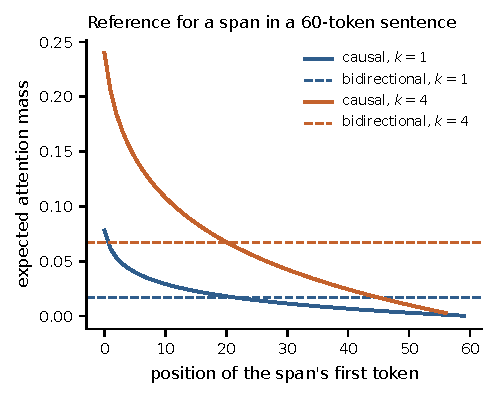
\includegraphics[width=0.6\linewidth]{img/fig_null.pdf}
  \caption{The attention an indifferent model would give a span in a 60-token sentence, as a function of where the span
  starts. Dashed: bidirectional reference (\cref{eq:null}), which depends only on the span's size $k$. Solid: causal
  reference (\cref{eq:closed}), which also depends on position. Computed from the formulas; no data.}
  \label{fig:null}
\end{figure}

Because every later comparison rests on these references, we verified them
numerically with the same functions the analysis uses to measure attention. We drew attention tensors whose rows are far
from uniform (gamma-distributed weights), and then, \nullPerm{} times, permuted each row's weights among the positions that
row may see. A permutation is exactly the indifferent model: each row keeps its values, and only which positions hold them
changes. Across \nullConfigs{} combinations of sentence length, span size and position, the mean measured mass matched
the reference to within \nullBidMaxZ{} standard errors for the bidirectional case and \nullCauMaxZ{} for the causal one.

With the reference we can remove geometry from attention and see what is left.
We use two versions: the \emph{enrichment} $m(S)/\mathbb{E}[m(S)]$, equal to 1 when an entity receives exactly its share and
above 1 when the model singles it out; and the \emph{geometric residual}, what remains of $m(S)$ after a linear regression on
$\mathbb{E}[m(S)]$. If the model's attention to an entity carries information about whether the extraction is correct, it
should appear in these deconfounded scores. The two versions remove geometry in different ways. Enrichment is a ratio and places every
entity on the same relative scale; the residual is a difference and keeps the absolute amount of attention. Using both guards
against a conclusion that depends on how geometry was removed.

\subsection{What attention has to beat}
\label{sec:scores}

Attention is only worth reading if it adds to what the extractor already reports, its confidence. For
\gliner{} the confidence is the probability the model assigns to the (span, label) pair, a sigmoid output for each pair. For the
decoders it is the geometric mean of the probabilities of the tokens generated for the mention and its label.

The decoders' own probability is known to be a weak estimate of span
correctness, so we also compare with AggSeq~\citep{hashimoto2024beam}: we decode five beams, weight each by its
length-normalised probability renormalised over the five, and give each predicted pair the total weight of the beams that
contain it. Attention would have to beat both.

To see how much of attention's ranking can be obtained without looking at attention, we
also rank by the span length $k$, the sentence length $T$, and the geometric fraction itself. None of these needs anything from
inside the model. They bound what attention can claim: if a ranking that never looks inside the
model does as well as attention, whatever attention offers can be had without it.

The practically relevant question is whether attention improves confidence when the two are used together. We standardise both with the mean and standard deviation of the calibration part, combine them as
$w\,z_{\text{att}}+(1-w)\,z_{\text{conf}}$, choose $w$ among $\{0,0.01,\dots,1\}$ to minimise the \aurc{} on calibration, and
apply that $w$ to the evaluation part. Standardising puts the two scores on one scale, so that $w$ measures their relative contribution rather
than their units. The test is deliberately generous to attention: the procedure is free to give it any weight,
including all of it. If attention held information confidence lacks, the chosen weight would reflect it. A weight of exactly zero
means the procedure preferred confidence alone.

\subsection{Protecting the comparisons from our choices}
\label{sec:guard}

A negative result invites the objection that a different choice would have found the signal. We answered this in two ways.

Every comparison in this paper, with its estimator and its decision rule, was written down
before the measurement it concerns: which layers and heads to average, how to treat the first token, which scores to compare and
what counts as an improvement. This prevents the analysis from being adapted to the result (Appendix~\ref{app:protocol}).

A declared choice can still be the wrong one. We therefore evaluated, for \gliner{}
base on the validation partition, \periReadings{} readings per corpus: four directions (attention received, attention the span pays
to itself, their mean, and attention received per token), three treatments of the first token, sixteen selections of layers (all
together, each alone, and three ranges) and thirteen selections of heads (all together and each alone). The point of this scan is
not to find the best reading, which would be selecting on the data, but to see whether any reasonable reading behaves differently.

\subsection{Extractors and data}
\label{sec:setup}

We use two corpora whose entities differ in kind: GENIA~\citep{Kim2003genia}, biomedical abstracts whose entities are often long
multi-word terms (\nSentGenia{} test sentences), and CoNLL-2003~\citep{tjongkimsang2003conll}, newswire with short names of people,
places and organisations (\nSentConll{}). We use three bidirectional extractors, so that the conclusion is not tied to a single model:
\gliner{} base and large~\citep{Zaratiana2024gliner}, and \gliner{} base fine-tuned on each corpus, which raises validation F1 from
\ftFoneGeniaBefore{} to \ftFoneGeniaAfter{} on GENIA and from \ftFoneConllBefore{} to \ftFoneConllAfter{} on CoNLL-2003. Fine-tuning asks whether a weak signal is merely a symptom of an extractor that fits the
corpus poorly: an adapted extractor makes fewer errors, and a signal about its errors should, if anything, become easier to see. To test a
different architecture we add two causal extractors, Qwen2.5 with 0.5B and 1.5B parameters~\citep{qwen2025}, fully fine-tuned on each
corpus to write out mentions and labels and decoded greedily. The decoders address the two objections a single architecture leaves open: that the result
belongs to bidirectional attention, and that it belongs to small models. The causal mask changes the reference, and the two
sizes differ by a factor of three in parameters. All values are on the test partition unless stated.

% ============================================================================
\section{Results}
\label{sec:results}

We present the results in the order of the questions that produced them. Each step answers one question and raises the next.

\subsection{How much of the attention an entity receives is geometry?}
\label{sec:res-geometry}

The first measurement showed attention removing \rrGeniaMassBase\% of the risk on GENIA. Before
interpreting that number we needed to know how much of the attention an entity receives is simply its share of the budget.

Nearly all of it turned out to be that share. For the three bidirectional extractors, the geometric fraction of \cref{eq:null}
explains the attention mass with $R^2$ between \encRsqMin{} and \encRsqMax{} (\cref{tab:aurc}); for the decoders, the causal
reference of \cref{eq:nullcausal} explains \decRsqMin--\decRsqMax{} of it. The deviations from the reference also have a consistent
direction: the median entity receives only \encObsExpMin--\encObsExpMax{} of its geometric share. The model does not single entities
out; if anything, it attends to them less than their size alone would predict.

This was not yet the answer, because two quantities can be closely correlated and still rank errors differently, because
ranking depends on the small differences a correlation averages over. The residual variance could hold exactly the error signal we
were looking for. So the question that mattered was not how similar attention and geometry are, but whether they rank errors
differently.

The decisive comparison is in \cref{fig:mechanism}. For every extractor and corpus it plots how well the
geometric fraction ranks errors against how well attention does, both relative to chance. The points fall on the diagonal. For the
bidirectional extractors, the two rankings produce the same \aurc{} to within \encMassGeoMaxGap{}, on both corpora. They beat chance
together on GENIA and lose to it together on CoNLL-2003. The decoders fall on the same line. Whatever attention contributed to the
\rrGeniaMassBase\% we started from, the lengths of the span and the sentence contributed as well, without the model.

\begin{figure}[t]
  \centering
  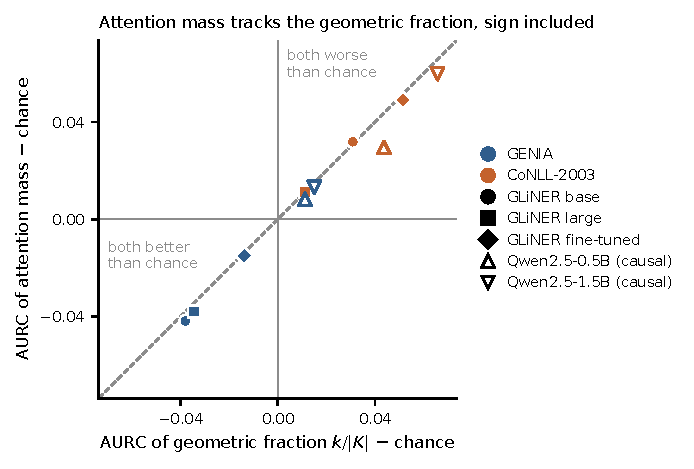
\includegraphics[width=0.78\linewidth]{img/fig_mechanism.pdf}
  \caption{Attention ranks errors as the geometric fraction does. Each point is one extractor on one corpus. Both axes show
  \aurc{} minus the \aurc{} of random abstention, so negative values are better than chance. Horizontal: ranking by the geometric
  fraction (\cref{eq:null,eq:nullcausal}), which uses no attention. Vertical: ranking by the attention mass received
  (\cref{eq:mass}). Dashed line: identity. Filled markers: bidirectional \gliner; open markers: causal Qwen2.5.}
  \label{fig:mechanism}
\end{figure}

\begin{table}[t]
\centering
\small
\caption{\aurc{} on the test partition (lower is better). Chance is random abstention and equals the error rate. Span length and
geometric fraction use no attention. $R^2$: attention mass against the geometric fraction.}
\label{tab:aurc}
\setlength{\tabcolsep}{4pt}
\begin{tabular}{llcccccc}
\toprule
extractor & corpus & chance & \shortstack{span\\length} & \shortstack{geometric\\fraction} & \shortstack{attention\\mass} & confidence & $R^2$ \\
\midrule
\gliner{} base      & GENIA & \encBaseGeniaChance & \encBaseGeniaSize & \encBaseGeniaGeo & \encBaseGeniaMass & \encBaseGeniaConf & \encBaseGeniaRsq \\
                    & CoNLL & \encBaseConllChance & \encBaseConllSize & \encBaseConllGeo & \encBaseConllMass & \encBaseConllConf & \encBaseConllRsq \\
\gliner{} large     & GENIA & \encLargeGeniaChance & \encLargeGeniaSize & \encLargeGeniaGeo & \encLargeGeniaMass & \encLargeGeniaConf & \encLargeGeniaRsq \\
                    & CoNLL & \encLargeConllChance & \encLargeConllSize & \encLargeConllGeo & \encLargeConllMass & \encLargeConllConf & \encLargeConllRsq \\
\gliner{} fine-tuned& GENIA & \encTunedGeniaChance & \encTunedGeniaSize & \encTunedGeniaGeo & \encTunedGeniaMass & \encTunedGeniaConf & \encTunedGeniaRsq \\
                    & CoNLL & \encTunedConllChance & \encTunedConllSize & \encTunedConllGeo & \encTunedConllMass & \encTunedConllConf & \encTunedConllRsq \\
\midrule
Qwen2.5-0.5B        & GENIA & \decSmallGeniaChance & \decSmallGeniaSize & \decSmallGeniaGeo & \decSmallGeniaMass & \decSmallGeniaConf & \multirow{4}{*}{\decRsqMin--\decRsqMax} \\
                    & CoNLL & \decSmallConllChance & \decSmallConllSize & \decSmallConllGeo & \decSmallConllMass & \decSmallConllConf & \\
Qwen2.5-1.5B        & GENIA & \decLargeGeniaChance & \decLargeGeniaSize & \decLargeGeniaGeo & \decLargeGeniaMass & \decLargeGeniaConf & \\
                    & CoNLL & \decLargeConllChance & \decLargeConllSize & \decLargeConllGeo & \decLargeConllMass & \decLargeConllConf & \\
\bottomrule
\end{tabular}
\par\smallskip{\footnotesize Decoder: causal reference (\cref{eq:nullcausal}); $R^2$ is the range over the four points.}
\end{table}

The equivalence is looser within entities of the same size. Over all entities, the geometric fraction mixes two lengths. Within a group of entities of the same size $k$ it reduces to $k/|K|$ with $k$ fixed, that is, to a ranking by
sentence length alone, and the comparison becomes stricter: among entities of equal size, does attention rank errors
differently from sentence length? \Cref{tab:strata}(a) shows that it sometimes does. Across the \strataCtwoN{} intervals
for strata of span size and nesting, attention ranks better than the geometric fraction in \strataCtwoFav{} and worse in
\strataCtwoAdv{}, where chance would give about \strataCtwoChance{} of each, by up to \strataCtwoMaxAbs{} in \aurc. The
direction is not consistent: attention does better for medium-sized entities on GENIA with the base and large extractors,
and for single-token entities with the extractor fine-tuned on GENIA, but worse for several strata on CoNLL-2003. Within a
size class, then, attention carries some information about correctness that sentence length does not. Whether that
information is new relative to the model's confidence is the question of \cref{sec:res-confidence}.

\begin{table}[t]
\centering
\small
\caption{Differences in \aurc{} by stratum, on the test partition (negative is better for the first term). Bold with
$\downarrow$: the 95\% interval lies below zero; $\uparrow$: above zero. (a) Attention mass against the geometric fraction.
(b) Confidence combined with deconfounded attention against confidence alone; 0 means the chosen weight on attention was
exactly zero. CoNLL-2003 has no nested entities.}
\label{tab:strata}
\setlength{\tabcolsep}{5pt}
% GENERATED by numeros.py. Do not edit.
\begin{tabular}{lcccccc}
\toprule
 & \multicolumn{3}{c}{GENIA} & \multicolumn{3}{c}{CoNLL-2003} \\
\cmidrule(lr){2-4}\cmidrule(lr){5-7}
stratum & base & large & fine-tuned & base & large & fine-tuned \\
\midrule
\multicolumn{7}{l}{\emph{(a) attention mass minus geometric fraction}} \\
$k=1$ & $-$0.009 & $-$0.004 & \textbf{$-$0.049}$^{\downarrow}$ & $+$0.009$^{\uparrow}$ & \textbf{$-$0.018}$^{\downarrow}$ & $-$0.002 \\
$k=2$ & \textbf{$-$0.024}$^{\downarrow}$ & \textbf{$-$0.025}$^{\downarrow}$ & $-$0.004 & $+$0.009$^{\uparrow}$ & $+$0.003 & $-$0.006 \\
$k=3$--$4$ & \textbf{$-$0.020}$^{\downarrow}$ & \textbf{$-$0.014}$^{\downarrow}$ & $-$0.003 & $+$0.004 & $+$0.010$^{\uparrow}$ & $+$0.001 \\
$k\ge5$ & $+$0.005 & $+$0.003 & $-$0.001 & $+$0.009 & $+$0.039$^{\uparrow}$ & $+$0.018$^{\uparrow}$ \\
nested & $+$0.009 & $+$0.008 & $+$0.032$^{\uparrow}$ & --- & --- & --- \\
flat & \textbf{$-$0.004}$^{\downarrow}$ & $-$0.003 & $-$0.002 & $+$0.001 & 0.000 & $-$0.003 \\
all & \textbf{$-$0.004}$^{\downarrow}$ & \textbf{$-$0.004}$^{\downarrow}$ & $-$0.001 & $+$0.001 & 0.000 & $-$0.002 \\
\midrule
\multicolumn{7}{l}{\emph{(b) confidence $+$ deconfounded attention, minus confidence}} \\
$k=1$ & 0 & $+$0.006 & $-$0.006 & \textbf{$-$0.003}$^{\downarrow}$ & \textbf{$-$0.014}$^{\downarrow}$ & 0 \\
$k=2$ & 0 & $-$0.003 & $+$0.007 & $+$0.001 & $+$0.002 & 0 \\
$k=3$--$4$ & 0 & $-$0.005 & 0.000 & $+$0.001 & $+$0.001 & 0 \\
$k\ge5$ & 0 & $+$0.001 & $+$0.002 & $+$0.002 & $+$0.005$^{\uparrow}$ & 0 \\
nested & 0 & $+$0.008 & $+$0.005 & --- & --- & --- \\
flat & 0 & $+$0.006 & $+$0.002 & 0.000 & $-$0.001 & 0 \\
all & 0 & $+$0.007$^{\uparrow}$ & $+$0.002 & 0.000 & $-$0.001 & 0 \\
\bottomrule
\end{tabular}

\end{table}

This left one question open: if attention is geometry, the sign of its usefulness should come from somewhere other than the
model. On CoNLL-2003, ranking by attention was worse than random. That is difficult to explain for a signal about the model's
errors, and it was the next thing to understand.

\subsection{Why does the same signal help on one corpus and hurt on the other?}
\label{sec:res-corpus}

The explanation was testable: if attention behaves like the geometric fraction, its sign should be predictable from how the two
lengths that define the fraction---the span's and the sentence's---relate to correctness in each corpus, without looking at
attention at all.

To check, we ranked the predictions by span length alone and by sentence length alone, and measured how much of
the risk each removes (\cref{eq:rho}). These two rankings tell us what the geometric fraction, which grows with the first and
shrinks with the second, will inherit.

For the three \gliner{} extractors, the corpora differ in exactly the way that explains the reversal
(\cref{fig:risk}). On GENIA, longer entities are more often correct, and ranking by span length
removes \rrSizeGeniaMin--\rrSizeGeniaMax\% of the risk, while sentence length is nearly uninformative
(\rrSentGeniaMin--\rrSentGeniaMax\%). The geometric fraction is then dominated by span length and helps
(\rrGeoGeniaMin--\rrGeoGeniaMax\%). On CoNLL-2003 the informative length is the sentence's: predictions in longer sentences are
more often correct, and sentence length alone removes \rrSentConllMin--\rrSentConllMax\% of the risk, while span length is
inconsistent across extractors ($\rrSizeConllMin$ to $\rrSizeConllMax$\%). Because the geometric fraction divides by the sentence
length, it places entities from \emph{short} sentences at the top of the ranking---precisely the ones more often wrong---and it is
worse than random for all three extractors ($\rrGeoConllMin$ to $\rrGeoConllMax$\%). Attention follows it.

The decoders make the same point from the other side. On GENIA their long predictions are \emph{not} more often correct: ranking
by span length is slightly worse than chance (\cref{tab:aurc}). Accordingly, the causal fraction does not help there either, and
neither does attention; both are worse than chance on both corpora. The relation that sets the sign belongs to the predictions
being ranked, which depend on the corpus and on the extractor, and attention follows it in every case.

In other words, the same model, reading the same kind of entities, can appear to have informative or harmful attention
depending only on how lengths are distributed among its correct and incorrect predictions on the test corpus. This also reconciles our result with
reports that attention predicts errors: on a corpus where the correct entities are the long ones, attention will look useful. In both
cases the signal comes from the data, and attention reflects it because each of its rows is a distribution.

Geometry explains attention's ranking on average, but the model could still attend to some entities
more or less than their share for reasons related to their correctness. The residual is small, but it is the part that would matter in
practice. The next question was whether it adds anything to the extractor's confidence.

\subsection{Once geometry is set aside, does attention add anything to confidence?}
\label{sec:res-confidence}

Confidence is the bar any score must clear, because it is free: the extractor already reports it. The
question is whether attention, and in particular attention with geometry removed, improves on it.

On its own, attention is far below confidence, as \cref{fig:risk} shows by placing every reading of attention next to confidence and to the lengths. Confidence removes \rrEncConfMin--\rrEncConfMax\% of the risk for \gliner{} and \rrDecConfMin--\rrDecConfMax\% for
Qwen2.5. Attention mass removes between $\rrEncMassMin$ and \rrEncMassMax\% for \gliner{} and between $\rrDecMassMin$ and
$\rrDecMassMax$\% for Qwen2.5. In all \nAttCells{} combinations of extractor and corpus, every attention summary falls at least
\rrAttBelowConfMin{} percentage points short of confidence. The strongest of them, the causal row entropy on CoNLL-2003, removes
\rrDecEntConllMin--\rrDecEntConllMax\% against \rrDecConfConllMin--\rrDecConfConllMax\% for confidence.

\begin{figure}[t]
  \centering
  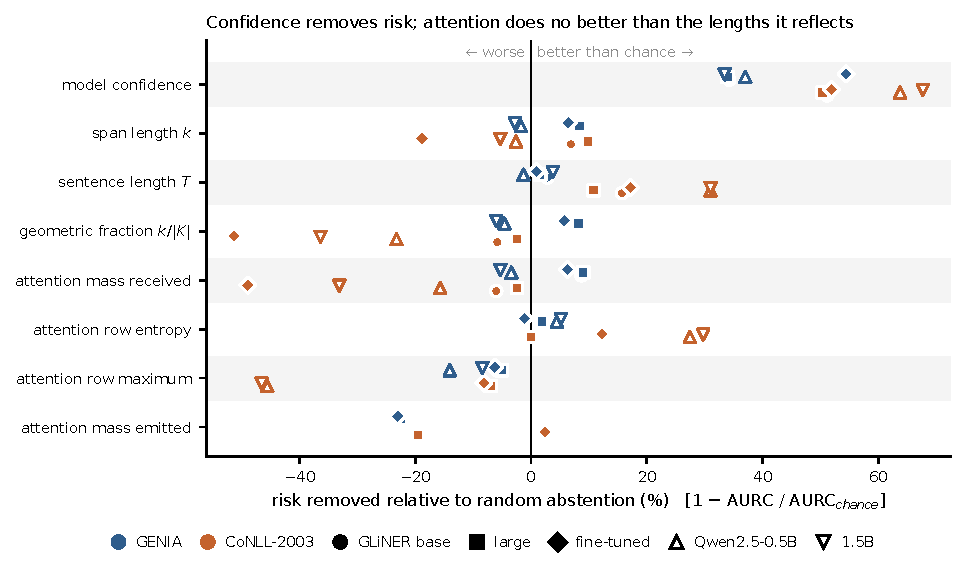
\includegraphics[width=\linewidth]{img/fig_risk.pdf}
  \caption{Share of the risk of random abstention removed by each score (\cref{eq:rho}), for each extractor and corpus, on the test
  partition. Top row: the model's confidence. Next three rows: scores that need nothing from inside the model. Last four rows: readings
  of attention (\cref{sec:reading}). Row entropy, row maximum and mass emitted were measured for \gliner{} large and fine-tuned, not for
  base; for Qwen2.5 the first two use their causal versions, and mass emitted is not defined.}
  \label{fig:risk}
\end{figure}

A weak signal can still help a strong one if it carries
different information. This is what the combination of \cref{sec:scores} tests, with the procedure free to give attention any weight.
The combination of confidence with deconfounded attention changes the \aurc{} of confidence by at most \cthreeMaxAbs, about
\cthreeMaxRel\% of its value, and in \cthreeZeroPairs{} of the \cthreePairs{} combinations of extractor and corpus the chosen weight on
attention is exactly zero. In deployment terms, for the extractor fine-tuned on GENIA, reaching 90\% precision requires reviewing
\loadTunedGeniaConf\% of the predictions when they are ranked by confidence and \loadTunedGeniaMass\% when they are ranked by attention:
no prefix of the attention ranking reaches that precision.

Pooled results can hide a group of entities for which attention helps, and within entities of the same size a trace does appear in the untuned extractors. \Cref{tab:strata}(b) repeats the combination within each stratum. Of the
\strataCthreeN{} stratum intervals, \strataCthreeFav{} improve on confidence, against about \strataCthreeChance{} expected by
chance, and \strataCthreeAdv{} is worse. Both improvements concern single-token entities on CoNLL-2003, for \gliner{} base
($\Delta\aurc=\cthreeKoneConllBaseD$) and large ($\cthreeKoneConllLargeD$). For the extractor fine-tuned on CoNLL-2003 the
procedure puts no weight on attention in any stratum. The within-size information of \cref{sec:res-geometry} is, for the
most part, already in the confidence; where it is not, it belongs to extractors that have not been adapted to the corpus.

The small residual we found belonged to the weaker extractors. There was one place where raw attention did slightly better than the
geometric fraction: GENIA, for \gliner{} base ($\Delta\aurc=\ctwoGeniaBaseD$, $[\ctwoGeniaBaseLo, \ctwoGeniaBaseHi]$) and large
($\ctwoGeniaLargeD$, $[\ctwoGeniaLargeLo, \ctwoGeniaLargeHi]$). For the extractor fine-tuned on GENIA the difference disappears
($\ctwoGeniaTunedD$, $[\ctwoGeniaTunedLo, \ctwoGeniaTunedHi]$). Whatever attention carried beyond the entity's size, a better-trained
extractor no longer shows it.

\subsection{Could the conclusion be an artefact of our choices?}
\label{sec:res-escapes}

A negative result is only as strong as the objections it withstands. At this point four were natural, and we tested each.

One objection is that attention was read the wrong way. We averaged all layers and heads, and read the attention an entity receives. Perhaps
the signal lives in one layer, one head, or in the attention the entity pays. Across the \periReadings{} readings of \cref{sec:guard},
each combined with confidence on validation data, the chosen weight on attention was exactly zero in \periGeniaZeroWeight\% of readings
on GENIA and \periConllZeroWeight\% on CoNLL-2003. Each weight is fitted on one part of the validation data and evaluated on the other, so each reading is judged out of
sample; only the choice of the best reading among thousands is optimistic. \Cref{fig:readings} shows the whole
distribution. On CoNLL-2003 almost every reading changes nothing. On GENIA most readings improve confidence slightly: the
median change is $\periGeniaMedDelta$ and a quarter of the readings improve it by more than \periGeniaQuartDeltaAbs. The
best reading changed the \aurc{} of confidence by $\periGeniaBestDelta$ on GENIA and $\periConllBestDelta$ on CoNLL-2003.
These are the numbers of \gliner{} base, the weakest extractor, whose residual disappears after fine-tuning.

\begin{figure}[t]
  \centering
  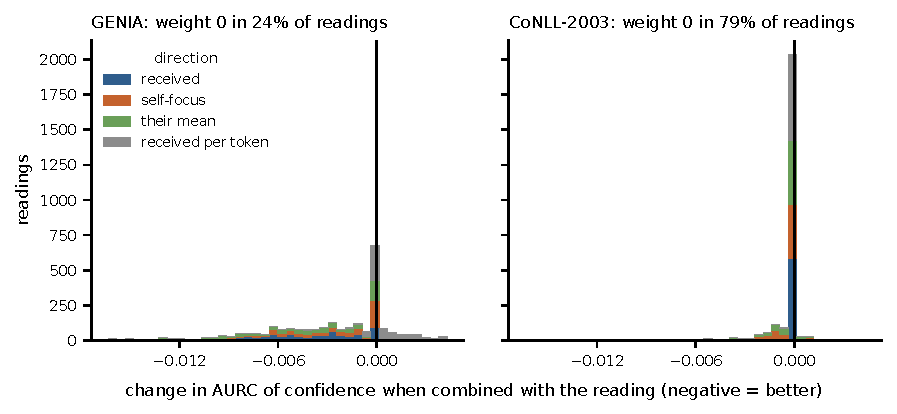
\includegraphics[width=\linewidth]{img/fig_readings.pdf}
  \caption{Change in the \aurc{} of confidence when it is combined with each of the \periReadings{} readings of attention of
  \gliner{} base, on the validation partition (weight fitted on one part, change measured on the other). Colours: which
  attention is read (\cref{sec:guard}). Negative values mean the combination beats confidence alone.}
  \label{fig:readings}
\end{figure} The readings also share the confound: their median correlation
with span length is \periGeniaSizeCorr{} on GENIA and \periConllSizeCorr{} on CoNLL-2003.

A second objection is that the mass received is only one summary. The row entropy, row maximum and mass emitted, which describe the attention the
entity's own tokens pay, never improve on confidence in review load, for the large extractor (\famLargeAttFav{} of \famLargeAttN{}
intervals below zero) or for the fine-tuned ones (\famTunedAttFav{} of \famTunedAttN).

A third objection is that the extractor was too weak. Fine-tuning raised F1 substantially and, on GENIA, where the residual had appeared, removed it
rather than revealing more (\cref{sec:res-confidence}).

A last objection is that a bidirectional encoder is a special case. Causal decoders process text differently, and their reference is different
too (\cref{eq:nullcausal}). For Qwen2.5 at both sizes, the three attention signals are worse than confidence and worse than AggSeq in all
\decAttPooledN{} comparisons. Tripling the size of the model, from 0.5B to 1.5B parameters, changes none of them.

The stratified comparisons of \cref{sec:res-geometry,sec:res-confidence}, repeated for the decoders (\cref{tab:strata-dec}),
show where the causal case departs from the bidirectional one. Against the causal geometric fraction, the decoders' attention
ranks errors \emph{worse} for single-token mentions in all four models; these are the largest differences in the table and
the only ones shared by every model. Across the \decStrataCtwoN{} stratum intervals attention is worse in \decStrataCtwoAdv{}
and better in \decStrataCtwoFav{}.
Combined with confidence, attention receives no weight at all in \decStrataCthreeZeroW{} of the \decStrataCthreeN{} stratum
intervals, and improves on confidence in \decStrataCthreeFav{}, about the \decStrataCthreeChance{} expected by chance: single-token
mentions for the 1.5B model on GENIA, a stratum of 170 entities whose interval is wide. The decoders thus show no
counterpart to the trace found in the untuned encoders.

\begin{table}[t]
\centering
\small
\caption{The stratified comparisons of \cref{tab:strata}, for the Qwen2.5 decoders fine-tuned on each corpus. The reference in
(a) is the causal geometric fraction (\cref{eq:closed}). Notation as in \cref{tab:strata}.}
\label{tab:strata-dec}
% GENERATED by numeros.py. Do not edit.
\begin{tabular}{lcccc}
\toprule
 & \multicolumn{2}{c}{GENIA} & \multicolumn{2}{c}{CoNLL-2003} \\
\cmidrule(lr){2-3}\cmidrule(lr){4-5}
stratum & 0.5B & 1.5B & 0.5B & 1.5B \\
\midrule
\multicolumn{5}{l}{\emph{(a) attention mass minus causal geometric fraction}} \\
$k=1$ & $+$0.081$^{\uparrow}$ & $+$0.095$^{\uparrow}$ & $+$0.067$^{\uparrow}$ & $+$0.045$^{\uparrow}$ \\
$k=2$ & $+$0.013 & 0.000 & $+$0.004 & $-$0.001 \\
$k=3$--$4$ & $+$0.002 & $+$0.009 & 0.000 & $-$0.001 \\
$k\ge5$ & \textbf{$-$0.014}$^{\downarrow}$ & $-$0.006 & $-$0.005 & $+$0.010 \\
nested & $+$0.021 & $+$0.015 & --- & --- \\
flat & $+$0.005 & $+$0.008$^{\uparrow}$ & $+$0.025$^{\uparrow}$ & $+$0.018$^{\uparrow}$ \\
all & $+$0.009$^{\uparrow}$ & $+$0.011$^{\uparrow}$ & $+$0.025$^{\uparrow}$ & $+$0.018$^{\uparrow}$ \\
\midrule
\multicolumn{5}{l}{\emph{(b) confidence $+$ deconfounded attention, minus confidence}} \\
$k=1$ & 0 & \textbf{$-$0.061}$^{\downarrow}$ & 0 & 0 \\
$k=2$ & 0 & 0.000 & 0 & 0 \\
$k=3$--$4$ & 0 & $-$0.005 & 0 & 0 \\
$k\ge5$ & 0 & $+$0.010 & 0 & 0 \\
nested & 0 & $-$0.025 & --- & --- \\
flat & 0 & $+$0.001 & 0 & 0 \\
all & 0 & $-$0.001 & 0 & 0 \\
\bottomrule
\end{tabular}

\end{table}

% ============================================================================
\section{What the evidence establishes, and what else could explain it}
\label{sec:discussion}

The chain of results supports a specific conclusion. In entity extraction, the scalar summaries of attention one would first reach for
inform abstention largely through the geometric fraction, the share of the context an entity occupies. Their usefulness, and even its sign,
is inherited from how lengths relate to correctness among the predictions being ranked. What they carry beyond geometry is, with one small exception in extractors not adapted to the
corpus, already contained in the model's confidence.

The results do not show that the network holds no information about its errors. Several explanations remain compatible with what we
observed, and each suggests an experiment.

First, the confound may be a general property of corpora. If the sign of attention's apparent value is set by the relation between length
and correctness, it can be \emph{predicted} before attention is measured: on a new corpus, the risk removed by span length and by sentence length,
computed from the predictions alone, should tell whether attention will look helpful or harmful. This is the most direct test of the mechanism, and
it would turn the present analysis, run on two corpora, into a replication.

Second, errors are not all of one kind. A wrong prediction may have wrong boundaries, a wrong label, or no annotated counterpart. Attention
to an entity plausibly speaks to its boundaries and not to its label, and pooling all errors could hide a signal specific to one kind. This can be
tested without new measurements, since the error type follows from the annotations.

Third, the information may exist, but not in a scalar. Averaging over heads and layers, which our readings do, can destroy information
spread across them. A reader trained on per-head attention, given the geometric fraction as an input, would test this. It would give up the
exact reference, because its weights are fitted to the data. The same situation holds for hidden states and output scores, which have no exact
reference at all; we study them separately.

% ============================================================================
\section{Limitations}
\label{sec:limitations}

The evidence comes from one task, two corpora and extractors of up to 1.5B parameters. Confidence is defined differently for the two architectures,
so each is compared with its own confidence and never across them. The comparisons were declared before measurement, but in a private repository;
the released code verifies that each result follows from its declaration, not when the declaration was written. Past dates cannot be
established from a private history, and we do not claim them. To make the declarations verifiable from here on, the SHA-256 of every
declaration, addendum and executable configuration was deposited on Zenodo on \preregDate{} (\preregDOI); a single command checks the
released files against that deposit. Several declarations were made on the same two test sets, as each question followed from an earlier result;
a corpus not yet examined would turn the conclusions into a replication. Appendix~\ref{app:protocol} lists every departure from the declarations.

% ============================================================================
\section{Conclusion}
\label{sec:conclusion}

We began by asking whether the attention an extracted entity receives could tell a reviewer which predictions to check. It first appeared that it
could. Asking what attention a model would pay to an entity if it paid no particular attention to it led to an exact reference, and against that
reference the apparent signal turned out to be the share of the sentence the entity occupies. That share predicts correctness on one corpus and
anti-predicts it on the other, and attention followed it in both. With geometry set aside, attention added almost nothing to the extractor's own
confidence, whichever way we read it, whichever extractor we used, and whether the model was bidirectional or causal.

The practical lesson is simple, and the comparison that supports it costs nothing to run: before treating attention as evidence about an error,
compare it with the geometric fraction, which is computed from two lengths. Attention may not be explanation~\citep{jain-wallace-2019-attention},
and it may not not be explanation~\citep{wiegreffe-pinter-2019-attention}; for deciding when an extractor should abstain, it is, largely, geometry.

Code, declarations and measured tables (without corpus text) are available at \repoURL{},
archived as \codeDOI. Every number, table and figure in this paper is regenerated from them by a single command and compared byte for
byte with the published version. The six fine-tuned weights are archived under the licences they inherit, as \weightsDOIgliner{}
(GLiNER, CC-BY-NC-4.0) and \weightsDOIqwen{} (Qwen2.5, Apache-2.0), each with a content fingerprint that the
repository checks before any measurement.

\begin{acknowledgments}
This study was financed in part by the Coordenação de Aperfeiçoamento de Pessoal de Nível Superior -- Brasil (CAPES) --
Finance Code 001. Parts of the code, analyses and text were produced with an AI assistant under the authors' direction; the
authors reviewed all of it and take full responsibility.
\end{acknowledgments}

\bibliographystyle{plainnat}
\bibliography{references}

% ============================================================================
\appendix
\section{Pre-registration and analysis protocol}
\label{app:protocol}

The study was conducted under a series of declarations, each written as executable configuration before the measurement
it governs and hashed in two parts: what produces the measured table, and what analyses it. The analysis code refuses a declaration whose hash differs
from the signed document. Rules of the protocol are versioned, and each declaration is analysed under the rules of the version it was signed under.
This paper uses the declarations on attention; declarations on hidden states and output scores, measured in the same runs, are reported separately.

The declared comparisons used in this paper are the following. Descriptive: $R^2$ of attention mass against the reference, and the median of observed over expected.
Attention mass against the geometric fraction (\aurc). Confidence combined with enrichment against confidence (\aurc). Attention mass, enrichment, and
their combination with confidence against confidence (review load at each target precision). Row entropy, row maximum and mass emitted against
confidence (review load). For the decoders, the attention signals against confidence and against AggSeq. Each comparison is also reported by span
length ($k=1$, $2$, $3$--$4$, $\ge5$) and for nested versus flat entities.

When we count intervals, an interval is favourable when it lies below zero, adverse when above, and degenerate when both bounds are zero (the
combination chose weight zero, or neither score reaches the target). Under no difference, a non-degenerate interval is favourable with probability
0.025; intervals within a declaration share predictions, so this calibrates scale and is not a test. \Cref{fig:tallies} gives the count for every
declared comparison on attention.

\begin{figure}[h]
  \centering
  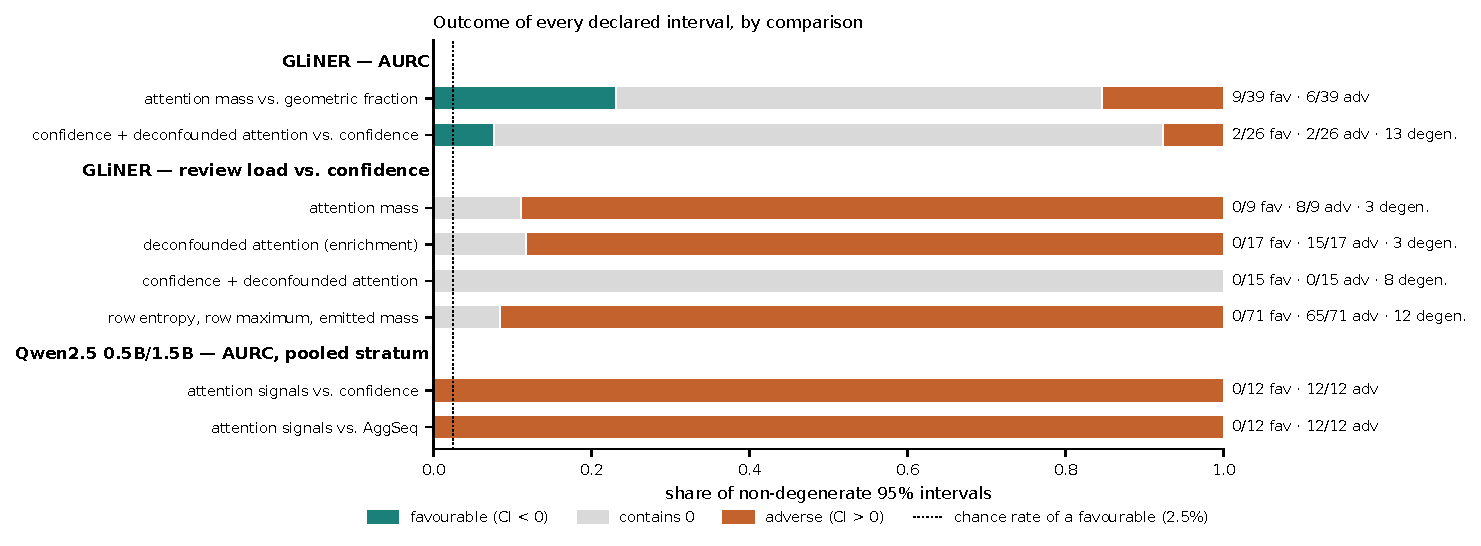
\includegraphics[width=\linewidth]{img/fig_tallies.pdf}
  \caption{Outcome of every declared interval on attention, by comparison. Counts to the right; dotted line: the 2.5\% chance rate of a favourable
  interval.}
  \label{fig:tallies}
\end{figure}

The departures from the declarations, in the order they occurred, were these:
\begin{itemize}
  \item The pilot (bootstrap over entities) preceded the adoption of the sentence-level bootstrap. Under the current analysis its estimates and
  verdicts are unchanged and its interval bounds move in the third decimal. It showed attention beating random abstention on GENIA
  ($\pilotFloorGeniaD$, $[\pilotFloorGeniaLo, \pilotFloorGeniaHi]$) and losing to it on CoNLL-2003 ($\pilotFloorConllD$,
  $[\pilotFloorConllLo, \pilotFloorConllHi]$).
  \item The row-summary declarations for the fine-tuned extractors were signed before, but measured after, the result of the same design on
  \gliner{} large was known.
  \item An addendum written after signature, and before any decoder result was computed, fixed which decoder quantity each name denotes, adopted
  the causal reference, and removed generated mentions absent from the input for every score alike.
  \item The exact-zero weights behind degenerate intervals depend on whether a score's direction is fixed on calibration data; the verdicts do not.
\end{itemize}

\end{document}
